\section{Simulation and Testing }

\begin{frame}
    \frametitle{Simulation Testing for Foundation DB}
    \begin{itemize}
        \item Testing and debugging distributed systems is challenging, particularly for Foundation DB (FDB).
        \item FDB employs an ambitious approach using a deterministic discrete-event simulation.
        \item The simulation environment quickly exposes bugs in the database, ensuring reproducibility for investigation.
    \end{itemize}
\end{frame}
%------------------------------------------------
\begin{frame}
    \frametitle{Deterministic Simulator}
    \begin{itemize}
        \item All database
code is deterministic and multithreaded concurrency is
avoided (instead, one database node is deployed per core).
        \item All sources of nondeterminism and communication are
abstracted, including network, disk, time, and pseudo-
random number generator
        \item Flow, a syntactic extension to C++, facilitates deterministic execution of highly concurrent code.
    \end{itemize}
\end{frame}
%------------------------------------------------
\begin{frame}
    \frametitle{Execution of the Simulator}
    \begin{itemize}
        \item Multiple FDB servers communicate through a simulated network in a single discrete-event simulation.
        \item Workloads written in Flow interact with simulated FDB servers.
    \end{itemize}
\end{frame}
%------------------------------------------------

\begin{frame}
    \frametitle{The FDB deterministic simulator}
    \begin{center}
        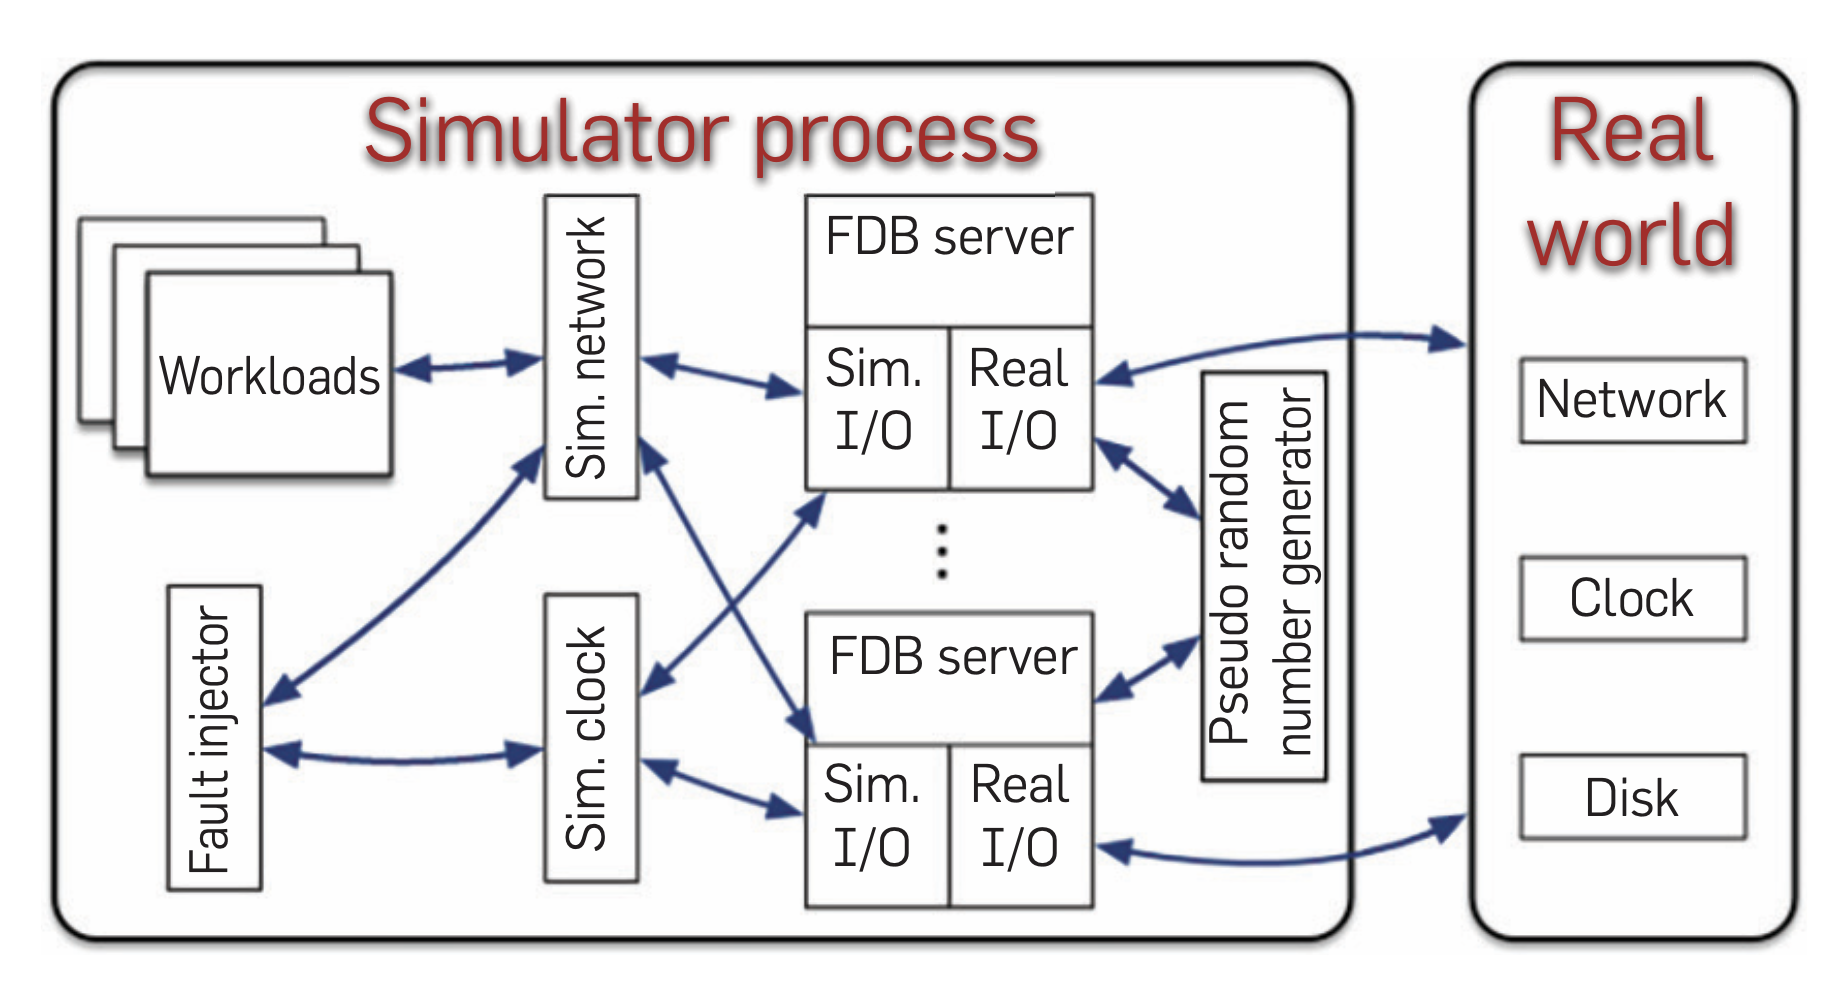
\includegraphics[width=0.8\textwidth]{img/3-Testing/The FDB deterministic simulator.png}
    \end{center}
    
\end{frame}


%------------------------------------------------
\begin{frame}
    \frametitle{Testing the system}
    \begin{itemize}
        \item FDB uses various test to detect failures in simulation.
        \item Assertions and invariants
in their data that can only be maintained through ATOMIC transaction and isolation built into synthetic workloads to verify database contracts and properties.
        \item Recoverability is checked by set of failures sufficient to break
the database’s availability.
    \end{itemize}
\end{frame}
%------------------------------------------------
\begin{frame}
    \frametitle{Fault Injection}
    \begin{itemize}
        \item Simulation injects various faults such as machine failures, network partitions, and disk behavior.
        \item Fault injection techniques test database resilience and increase simulation state diversity.
        \item FDB cooperates with the simulation to make rare states and events more common through "buggification", the simulation is allowed to inject some unusual (but not contractbreaking) behavior such as unnecessarily returning an
error from an operation that usually succeeds.
    \end{itemize}
\end{frame}
%------------------------------------------------
\begin{frame}
    \frametitle{Swarm Testing}
    \begin{itemize}
        \item Swarm testing maximizes simulation diversity by randomizing cluster size, workloads, fault injection parameters, and tuning parameters.
        \item Open-source swarm testing framework available for Foundation DB.
    \end{itemize}
\end{frame}
%------------------------------------------------
\begin{frame}
    \frametitle{Evaluation of Simulation Efficiency}
    \begin{itemize}
        \item Conditional coverage macros evaluate and tune simulation effectiveness.
        \item Quick bug discovery is crucial for testing and engineering productivity.
        \item Randomized testing and parallelization enhance code coverage and bug detection.
    \end{itemize}
\end{frame}
%------------------------------------------------
\begin{frame}
    \frametitle{Limitations of Simulation}
    \begin{itemize}
        \item Simulation may not reliably detect performance issues or test third-party dependencies.
        \item Bugs in critical dependent systems can lead to issues in FDB.
        \item Simulation cannot reliably detect performance issues, such as an imperfect load-balancing algorithm
    \end{itemize}
\end{frame}